\emph{Q$^{2}$ADPZ} (\textbf{Q}uite \textbf{A}dvanced \textbf{D}istributed \textbf{P}arallel \textbf{Z}ystem), es un sistema de computaci�n distribuida, multiplataforma y multiusuario para computadores de escritorio no dedicados dentro de una red TCP/IP. El poder de un gran n�mero de computadores ociosos es utilizado por usuarios que pueden ingresar tareas adem�s de monitorear su progreso. La flexibilidad del sistema implica varios modos en que las aplicaciones pueden ser ejecutadas. Tanto los programas de la tareas, los requerimientos de hardware y los archivos de entrada y salida son autom�ticamente manipulados por el sistema. Q$^{2}$ADPZ usa un protocolo de comunicaci�n interno basado en mensajes en formato XML.
\subsubsection{Caracter�sticas}
Los objetivos del dise�o de Q$^{2}$ADPZ son la facilidad de uso para diferentes niveles de conocimiento de los usuarios, operabilidad multiplataforma, arquitectura cliente-maestro-esclavo usando una r�pida comunicaci�n a base de mensajes, modularidad y adaptabilidad, seguridad de los computadores involucrados en el sistema, y sencillez en los procesos de instalaci�n y actualizaci�n.

En Q$^{2}$ADPZ, un peque�o programa (\emph{servicio esclavo}) corre en cada computador de escritorio. Mientras el computador no est� siendo utilizado, el servicio esclavo acepta tareas enviadas por el servidor (\emph{maestro}). El poder de c�mputo disponible es usado para ejecutar la tarea.
\subsubsection{Modos de uso}
El modo b�sico de uso de Q$^{2}$ADPZ es a trav�s de una aplicaci�n de l�nea de comando llamada \emph{cliente universal} y que le permite a los usuarios ingresar el programa a ejecutar. En este ingreso se puede especificar
\begin{itemize}
\item n�mero de ejecuciones del programa,
\item la ruta del ejecutable y los argumentos de l�nea de comando,
\item archivos de entrada y salida,
\item directorios donde residen los archivos,
\item utilidades a ser ejecutadas despu�s de las tareas individuales,
\item tiempo m�ximo asignado para la ejecuci�n de una tarea,
\item el orden en que los grupos de tareas ser�n ejecutados,
\item requerimientos de hardware (espacio en disco, memoria, velocidad y tipo de CPU) y software (sistema operativo y programas instalados).
\end{itemize}

Estos par�metros de configuraci�n son guardados en un archivo en formato XML. El ejecutable puede ser obtenido desde el disco local o descargado desde alguna direcci�n URL. Los archivos de entrada y salida son transferidos a los esclavos usando un servidor web dedicado a los datos.

Cada ejecuci�n corresponde a una tarea - la unidad de c�mputo m�s peque�a en Q$^{2}$ADPZ. Las tareas son agrupadas en trabajos - identificadas por un identificador y un nombre. El sistema permite la operaci�n de control sobre tareas, trabajos y usuarios. Usuarios avanzados pueden crear el archivo de configuraci�n manualmente o generarlo autom�ticamente.

Usuarios a�n m�s avanzados pueden prescindir del cliente universal y programar su propia \emph{aplicaci�n cliente}\footnote{user client application} que se comunique directamente con el maestro, permitiendo ingresar tareas din�micamente. Finalmente, los usuarios pueden programar sus propias \textit{bibliotecas esclavas}\footnote{user slave library} que en casos espec�ficos son, por lo general, m�s r�pidas que los programas ejecutables.


\subsubsection{Arquitectura}
El sistema consiste en un proceso central llamado \emph{maestro}, un n�mero variable de procesos en diferentes computadores de una red llamados \emph{esclavos} y un n�mero de procesos \emph{cliente} que generan tareas agrupadas en trabajos. En la figura \ref{fig:image01} se grafica este esquema.
\begin{figure}
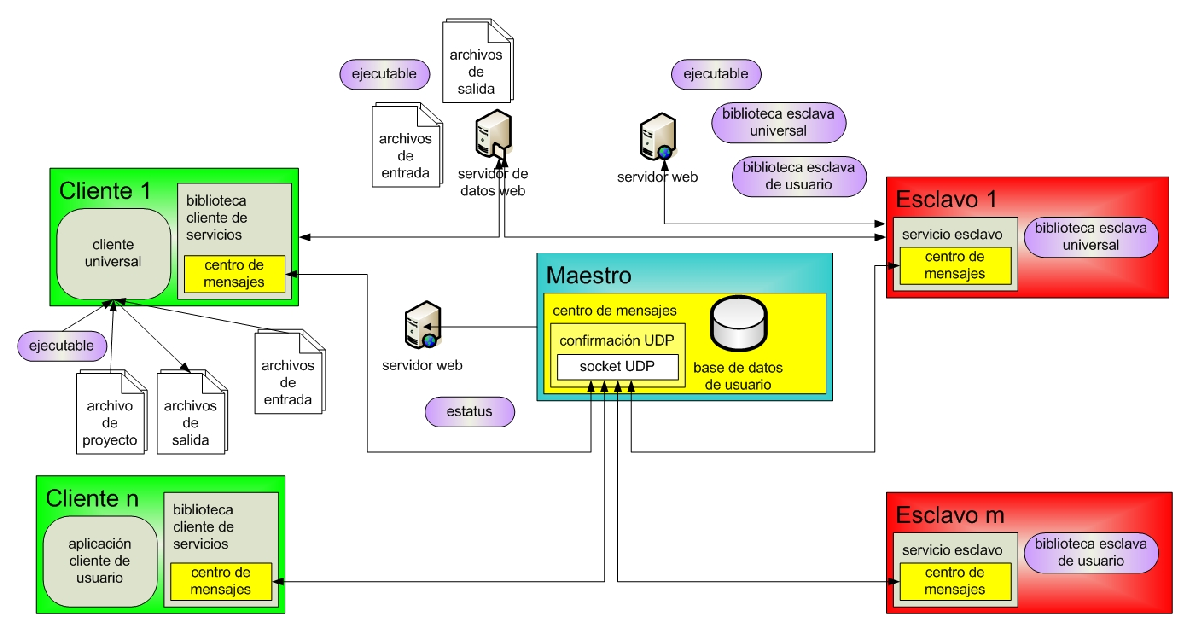
\includegraphics[width=\textwidth]{images/image01.eps}
\caption{La arquitectura de Q$^2$ADPZ}
\label{fig:image01}
\end{figure}
El componente esclavo corre como un proceso permanente. Su rol principal es notificar al \emph{maestro} sobre su estado y sus recursos disponibles. Otro rol que posee es lanzar una aplicaci�n, consecuencia de una petici�n del maestro. La aplicaci�n, en la forma de una biblioteca, ejecutable o programa interpretado, es transferida desde el servidor de acuerdo a la descripci�n de la tarea, entonces es ejecutada con los argumentos de l�nea de comando especificadas en dicha descripci�n.

Al momento en que un esclavo recibe una tarea, en primera instancia descarga el ejecutable o programa interpretado desde un repositorio autom�tico de datos (implementado sobre un servidor web en Perl), o desde una direcci�n URL. Luego, el esclavo procede a descargar y preparar todos los archivos de entrada requeridos. Despu�s que el ejecutable o programa interpretado termina, los archivos de salida generados son subidos al repositorio web para ser posteriormente obtenidos por el cliente que cre� la tarea.

El maestro adem�s escucha a todos los esclavos y de esta forma tiene una visi�n general de todos los recursos disponibles en el sistema. El maestro acepta peticiones de tareas de los clientes y le asigna los nodos (esclavos) m�s adecuados. Adem�s de esto, el maestro permite reservar nodos: los clientes son notificados despu�s de que los recursos se encuentren disponibles.

El cliente consiste en una aplicaci�n que usa una biblioteca cliente de servicios. Esta biblioteca provee una API C++ para la comunicaci�n con el maestro, permitiendo controlar y comenzar trabajos y tareas, adem�s de obtener los resultados de �stos. Los usuarios pueden utilizar la API directamente en sus aplicaciones o usar un cliente universal que ingresa y controla las tareas en base a un archivo de especificaci�n en formato XML.

\subsubsection{Comunicaci�n}
\begin{figure}
\begin{center}
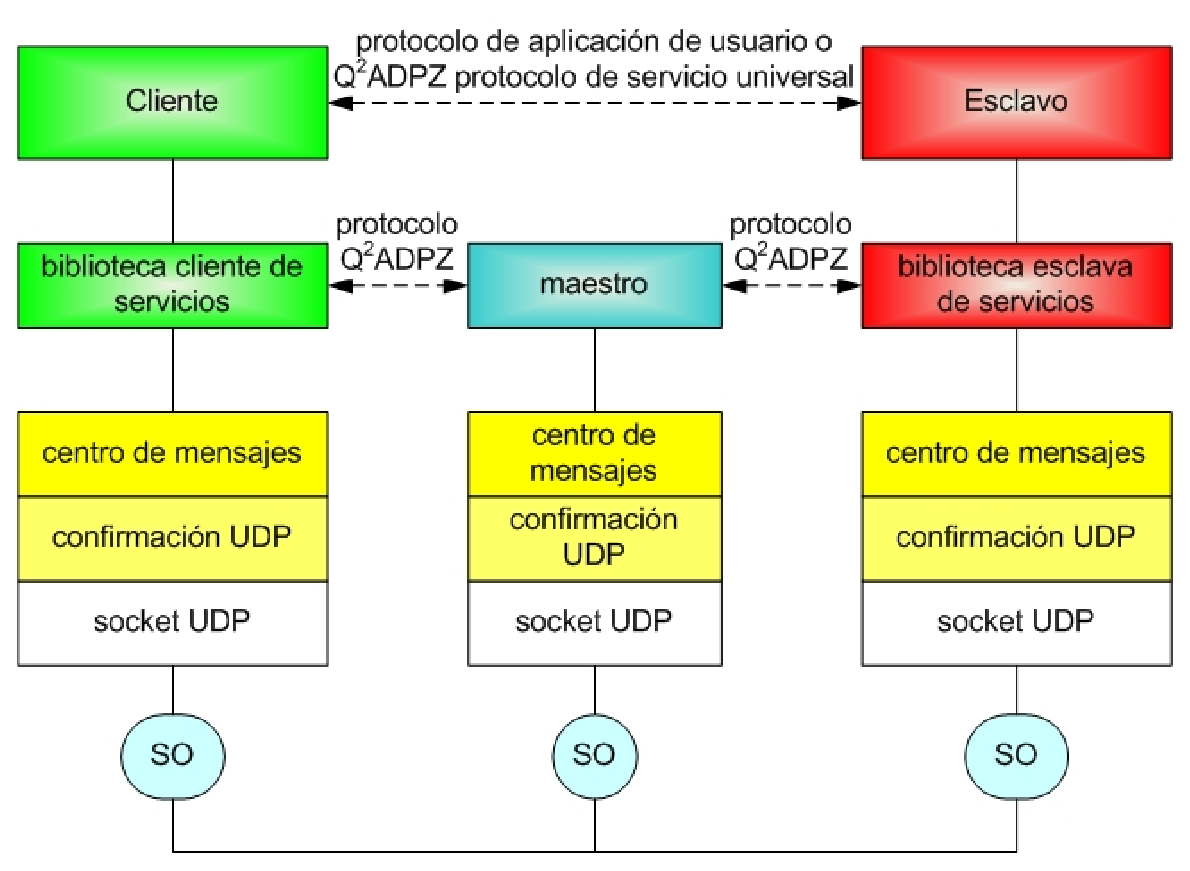
\includegraphics[width=0.7\textwidth]{images/image02.eps}
\end{center}
\caption{Las capas de comunicaci�n de Q$^2$ADPZ}
\label{fig:image02}
\end{figure}
La comunicaci�n en Q$^{2}$ADPZ est� basada en UDP, un protocolo de comunicaci�n poco fiable, en donde no est� garantizado que los paquetes enviados lleguen a su destino y si lo hacen, puede que no lleguen en el orden correcto. La ventaja de UDP sobre su alternativa, TCP, es su rapidez gracias a que carece de m�ltiples mecanismos enfocados en la conexi�n que implican una carga adicional a la comunicaci�n. Esta base conforma la primera capa de abstracci�n llamada \emph{socket UDP} que tiene como prop�sito la transmisi�n de mensajes de control usados dentro del sistema. Sobre esta base de comunicaci�n UDP, existe una capa superior de abstracci�n llamada \emph{confirmaci�n UDP}. El prop�sito de esta capa es darle m�s fiabilidad a UDP mediante mensajes de confirmaci�n para los mensajes enviados.

La siguiente capa es el \emph{centro de mensajes} que recibe y env�a mensajes de alto nivel - elementos XML. Estos mensajes son intercambiados en formato XML de acuerdo al protocolo definido para las comunicaciones cliente-maestro y maestro-esclavo. Esta capa es s�lamente utilizada para prop�sitos de control de las entidades del sistema. Para transferir los archivos necesarios para la ejecuci�n de tareas se utiliza el protocolo HTTP.  La figura \ref{fig:image02} grafica el modelo de comunicaci�n antes descrito.
\subsubsection{Desventajas}
Q$^{2}$ADPZ es un sistema muy similar al propuesto en este proyecto pero posee ciertas caracter�sticas que son poco deseables y otras con las que no cuenta. Estas caracter�sticas se nombran a continuaci�n:
\begin{itemize}
\item Q$^{2}$ADPZ maneja la transmisi�n de archivos mediante un servidor web HTTP simple. Lo que requiere la puesta en marcha de un servicio web anexo al del sistema en s�. Adem�s un simple directorio web, sin una estructuraci�n especial no es lo m�s apropiado para manejar grandes cantidades de archivos\cite{filesystem}, lo que hace que Q$^{2}$ADPZ no soporte el trabajo con grandes conjuntos de datos.
\item Q$^{2}$ADPZ no permite comunicaci�n de sus componentes a trav�s de NATs. Esto es cr�tico dada las arquitecturas de red que existen en la actualidad, en espec�fico con la que cuenta la red de la Universidad de Concepci�n.
\item La comunicaci�n de Q$^{2}$ADPZ se basa en mensajes en formato XML que son demasiado pesados puesto que a�ade una serie de tags a los datos que codifica, congestionando el flujo de red.
\end{itemize}